%\DeclareMathOperator{\tri}{tri} \DeclareMathOperator{\rect}{rect}
%\DeclareMathOperator{\sgn}{sgn} \DeclareMathOperator{\ramp}{ramp}
%\DeclareMathOperator{\sinc}{sinc}


\subsection{Exponenti\"ele functies}
%\maketitle
%\begin{itemize}
%\item Wat is een exponenti\"ele functie?
%\item Hoe ziet het functievoorschrift van een exponenti\"ele functie eruit?
%\item Welke rekenregels voor machten en wortels zijn er?
%\item Hoe lossen we exponenti\"ele vergelijkingen op?
%\item Hoe kan je een exponenti\"ele functie grafisch voorstellen?
%\item Hoe bepaal je het tekenverloop van een exponenti\"ele functie? 
%\end{itemize}


\begin{definitie}
De exponenti\"ele functie is van de vorm:
\begin{equation*}
	y=a^{x}\text{ met }a\in\mathbb{R}_{0}^{+}\setminus\{ 1\}\text{ en }x\in\mathbb{R}
\end{equation*}
$a$ noemen we het \textbf{grondtal}, en moet strikt positief
en verschillend van 1 zijn.

$x$ noemen we de \textbf{exponent}, en is een re\"eel getal.
\end{definitie}

\begin{voorbeeld}
\begin{eqnarray*}
4^{2}&=&16 \\
3^{-2}&=&\frac{1}{3^{2}}=\frac{1}{9} \\
5^{\frac{2}{3}}&=&\sqrt[3]{5^{2}} \\
5^{-\frac{3}{2}}&=&\frac{1}{5^{\frac{3}{2}}}=\frac{1}{\sqrt{5^{3}}}=\frac{1}{\sqrt{5^{2}.5}}=\frac{1}{5\sqrt{5}}\\
\sqrt{25}&=&5 \\
\sqrt[4]{10000}&=&10\\
\sqrt[5]{-32}&=&-2\\
\sqrt[3]{8}&=&2\\
\end{eqnarray*}
\end{voorbeeld}

\begin{opmerking}
De positieve tweedemachts- of vierkantswortel van 25 is 5, want $5>0$ en $5^{2}=25$, dit wordt genoteerd als ${\displaystyle \sqrt{25}=5}$.

En de negatieve tweedemachts- of vierkantswortel van 25 is -5, want
$-5 < 0$ en $(-5)^{2}=25$, dit wordt genoteerd als ${\displaystyle -\sqrt{25}=-5}$.

Ook je rekenmachine zal bij ${\displaystyle \sqrt{25}}$ als resultaat
5 geven. Verwar dit niet met het oplossen van de vergelijking $x^{2}=25$.
In dit geval zijn de twee oplossingen van de vergelijking: $x=\pm\sqrt{25}=\pm5$.
\end{opmerking}

\subsubsection{Bijzondere gevallen}
\begin{itemize}
\item De exponenti\"ele functie met grondtal $e$ ($e=2,718281828$) wordt
genoteerd als $y=e^{x}$.
\item $a^{0}=1$
\item $a^{1}=a$
\item Als $n$ even is spreekt men van een \emph{evenmachtswortel} ($\sqrt{\ }$,
$\sqrt[4]{\ }$, ...), is $n$ oneven dan spreekt men van een \emph{onevenmachtswortel}
($\sqrt[3]{\ }$, $\sqrt[5]{\ }$, ...).
\item Positieve re\"ele getallen hebben twee tegengestelde evenmachtswortels
en juist \'e\'en positieve onevenmachtswortel.
\item als $n$ even is, dan heeft elk re\"eel getal $a$ twee $n$\textsuperscript{de}
machtswortels die tegengesteld zijn, genoteerd door $-\sqrt[n]{a}$
en $+\sqrt[n]{a}$, of kortweg $\pm\sqrt[n]{a}$.
\item als $n$ oneven is, dan heeft elk re\"eel getal a juist \'e\'en $n$\textsuperscript{de}
machtswortel, genoteerd door $\sqrt[n]{a}$.
\item Als $n$ even is, dan hebben de negatieve getallen geen $n$\textsuperscript{de}
machtswortel; dus negatieve re\"ele getallen hebben geen (re\"ele) evenmachtswortel
en juist \'e\'en onevenmachtswortel welke negatief is.
\end{itemize}
Let op: worteltrekken is niet hetzelfde als het oplossen van een vergelijking:

\begin{tabel}{}
\begin{tabular}{c|c}
worteltrekken & vergelijking oplossen\\
\hline 
$\sqrt{4}=2$ & $\begin{array}{lll}
x^{2} & = & 4\\
x & = & \pm\sqrt{4}\\
x & = & \pm2
\end{array}$\\
\hline 
 &  $x_{1}=-2$ en $x_{2}=+2$\\
\end{tabular}
\end{tabel}


\subsubsection{Rekenregels}

\begin{tabel}{}
\begin{tabular}{l|l}
machten & wortels\\
\hline 
$a^{m}a^{n}=a^{m+n}$ & $\sqrt[m]{a}\cdot\sqrt[n]{a}=\sqrt[m\cdot n]{a^{m+n}}$\\
$\frac{a^{m}}{a^{n}}=a^{m-n}$ & $\sqrt[n]{a^{m}}=a^{\frac{m}{n}}$\\
$\left(\frac{1}{a}\right)^{n}=a^{-n}$ & $\sqrt[n]{a}=a^{\frac{1}{n}}$\\
$\left(a^{m}\right)^{n}=a^{m\cdot n}$ & $\sqrt[n]{\sqrt[m]{a}}=\sqrt[n\cdot m]{a}$\\
$\left(a\cdot b\right)^{n}=a^{n}\cdot b^{n}$ & $\sqrt[n]{a\cdot b}=\sqrt[n]{a}\cdot \sqrt[n]{b}$\\
$\left(\frac{a}{b}\right)^{n}=\frac{a^{n}}{b^{n}}$ & $\sqrt[n]{\frac{a}{b}}=\frac{\sqrt[n]{a}}{\sqrt[n]{b}}$\\
\end{tabular}
\end{tabel}


\begin{opmerking}
	\ \\
	\begin{itemize}
\item aangezien $1=\frac{a}{a}=a^{1-1}=a^{0}$ zie je waarom
we zeggen dat $a^{0}=1$.
\item formules met wortels kan je (gemakkelijk) terugvinden als je de wortelvorm
herschrijft d.m.v. machten:
\end{itemize}
\begin{equation*}
\sqrt[m]{a}.\sqrt[n]{a}=a^{\frac{1}{m}}.a^{\frac{1}{n}}=a^{\frac{1}{m}+\frac{1}{n}}=a^{\frac{m+n}{m.n}}=\sqrt[m.n]{a^{m+n}}
\end{equation*}
\begin{itemize}
\item laat je niet vangen: $\sqrt{a+b}\neq\sqrt{a}+\sqrt{b}$
\item een veel gebruikte bewerking is het wortelvrij maken van de noemen,
bv.: $\frac{1}{\sqrt{2}}=\frac{1}{\sqrt{2}}.\frac{\sqrt{2}}{\sqrt{2}}=\frac{\sqrt{2}}{2}.$
\end{itemize}
\end{opmerking}

\subsubsection{Oplossen van exponenti\"ele vergelijkingen}

\textbf{Algemeen}

In sommige opgaves kom je exponenti\"ele vergelijkingen tegen. Dit zijn
vergelijkingen waar de onbekende voorkomt in de exponent. Om exponenti\"ele
vergelijkingen vlot te kunnen oplossen, maak je best gebruik van onderstaand
stappenplan:

Stap 1: Noteer de vergelijking in haar standaardvorm: $ a^{f(x)}=c$
of $ a^{f(x)}=a^{g(x)}$ of $ a^{f(x)}=b^{g(x)}$ 

Stap 2: Laat op beide leden van de vergelijking een geschikte logaritmische
functie inwerken.

Stap 3: Stop de uitkomst in de opgave en controleer.

\begin{voorbeeld}

Los op: $8^{x-1}-4=0$
\begin{equation*}
 \begin{array}{rclr}
 8^{x-1}-4=0 &
	\iff & 8^{x-1} = 4 & \text{ (stap 1)}\\
	& \iff & 2^{3x-3} = 2^{2} & \text{ (zoek een verband tss 8, 4 en 2)}\\
	& \iff & \log2^{3x-3} = \log2^{2} & \text{ (stap 2)}\\
	& \iff & 3x-3 = 2 & \text{}\\
	& \iff & x = \frac{5}{3}
	\end{array}
\end{equation*}

In stap 3 controleer je dat $ 8^{\frac{5}{3}-1}-4=0$?
Dit is ok.

Opmerking: stap 2 kan je ook in gedachten doen, m.a.w. hoef je niet
op te schrijven.

\end{voorbeeld}
\begin{voorbeeld}
	
\begin{equation*}
a^{f(x)}=b^{g(x)}
\end{equation*}

Los op: $50\sqrt{0,1^{x}}=10^{x+1}\sqrt{2,5}$

\begin{equation*}
 \begin{array}{rclr}
 50\sqrt{0,1^{x}}=10^{x+1}\sqrt{2,5} & 
	\iff & 50.\left(0,1\right)^{\frac{x}{2}} = 10^{x+1}\sqrt{2,5} & \text{ (stap 1)}\\
	&\iff & 50.10^{-\frac{x}{2}} = 10^{x}.10.\sqrt{2,5} & \text{ (zoek een verband tss 0,1 en 10)}\\
	&\iff & 10^{-\frac{x}{2}}.10^{-x} = \frac{10.\sqrt{2,5}}{50} & \textrm{(zet alle factoren met x bij elkaar)}\\
	&\iff & 10^{-\frac{3}{2}x} = \sqrt{\frac{100.2,5}{2500}}\\
	&\iff & \log10^{-\frac{3}{2}x} = \log10^{-\frac{1}{2}} & \text{ (stap 2)}\\
	&\iff & -\frac{3}{2}x = -\frac{1}{2} & \text{}\\
	&\iff & x = \frac{1}{3} & 
	\end{array}
\end{equation*}

In stap 3 controleer je dat $ 50\sqrt{0,1^{\frac{1}{3}}}=10^{\frac{1}{3}+1}\sqrt{2,5}$? Dit is ok.

Opmerking: stap 2 kan je ook in gedachten doen, m.a.w. hoef je niet
op te schrijven.
\end{voorbeeld}


\begin{voorbeeld}
Los op:  \begin{equation*}
2^{2x}-3\cdot 2^{(x+2)}+36=0
\end{equation*}

\begin{equation*}
 \begin{array}{lr}
 2^{2x}-3\cdot 2^{(x+2)}+36 = 0 & \\
	 2^{2x}-3\cdot 2^{x}\cdot 2^{2}+36 = 0 & \\
	 2^{2x}-12\cdot 2^{x}+36 = 0 & \text{ (herken dat \ensuremath{ 2^{2x}=\left(2^{x}\right)^{2}}}) \\
 	 & \text{ stel }2^{x}=t\\
	 t^{2}-12\cdot t+36 = 0 & \text{ (los de vierkantsvgl op)}
	\end{array}
\end{equation*}

\begin{equation*}
t_{1\textrm{ en }2}=\frac{-(-12)\pm\sqrt{(-12)^{2}-4\cdot 1\cdot 36}}{2\cdot 1}=\frac{12\pm0}{2}=6
\end{equation*}

We zoeken niet $ t_{1\textrm{ en }2}$ maar wel de waarde van $x$. Dus: $ 2^{x}=t=6$ zodat $ x=\log_{2}6$.

Ook hier kan je terug controleren of de gevonden waarde van $x$ voldoet
aan de gegeven vergelijking. 

Merk op dat in dit geval hier $ t_{1}$ en $ t_{2}$ gelijk zijn, waardoor er slechts \'e\'en $x$-waarde is. Indien $ t_{1}\neq t_{2}$ dan vind je ook een $x_{1}$ en $ x_{2}$.

Tenslotte, als je een $t$-waarde vindt die negatief is, dan... bestaat
de bijhorende $x$-waarde niet. Je kan immer geen logaritme nemen
van een negatief getal.

\end{voorbeeld}

\subsubsection{De exponenti\"ele functie}

Grafische voorstelling
\begin{itemize}
	\item Het domein van de exponenti\"ele functie is $\mathbb{R}$.
	\item Het beeld van de exponenti\"ele functie is ${\displaystyle \mathbb{R}}_{0}^{+}$,
	dus alle strikt positieve getallen; de grafiek ligt boven de $x$-as.
	\item De punten $(0,1)$ en $(1,a)$ behoren steeds tot de exponenti\"ele
	functie ${\displaystyle f(x)=a^{x}}$.
	\item Als het grondtal $a>1$ is het een stijgende functie.
	\item Als het grondtal $0<a<1$ is het een dalende functie.
	\item De grafieken ${\displaystyle y=a^{x}}$ en ${\displaystyle y=\left(\frac{1}{a}\right)^{x}=a^{-x}}$
	zijn elkaars spiegelbeeld t.o.v. de $y$-as.
\end{itemize}

%TODO figuur vervangen
\begin{figure}[H]
	\begin{center}
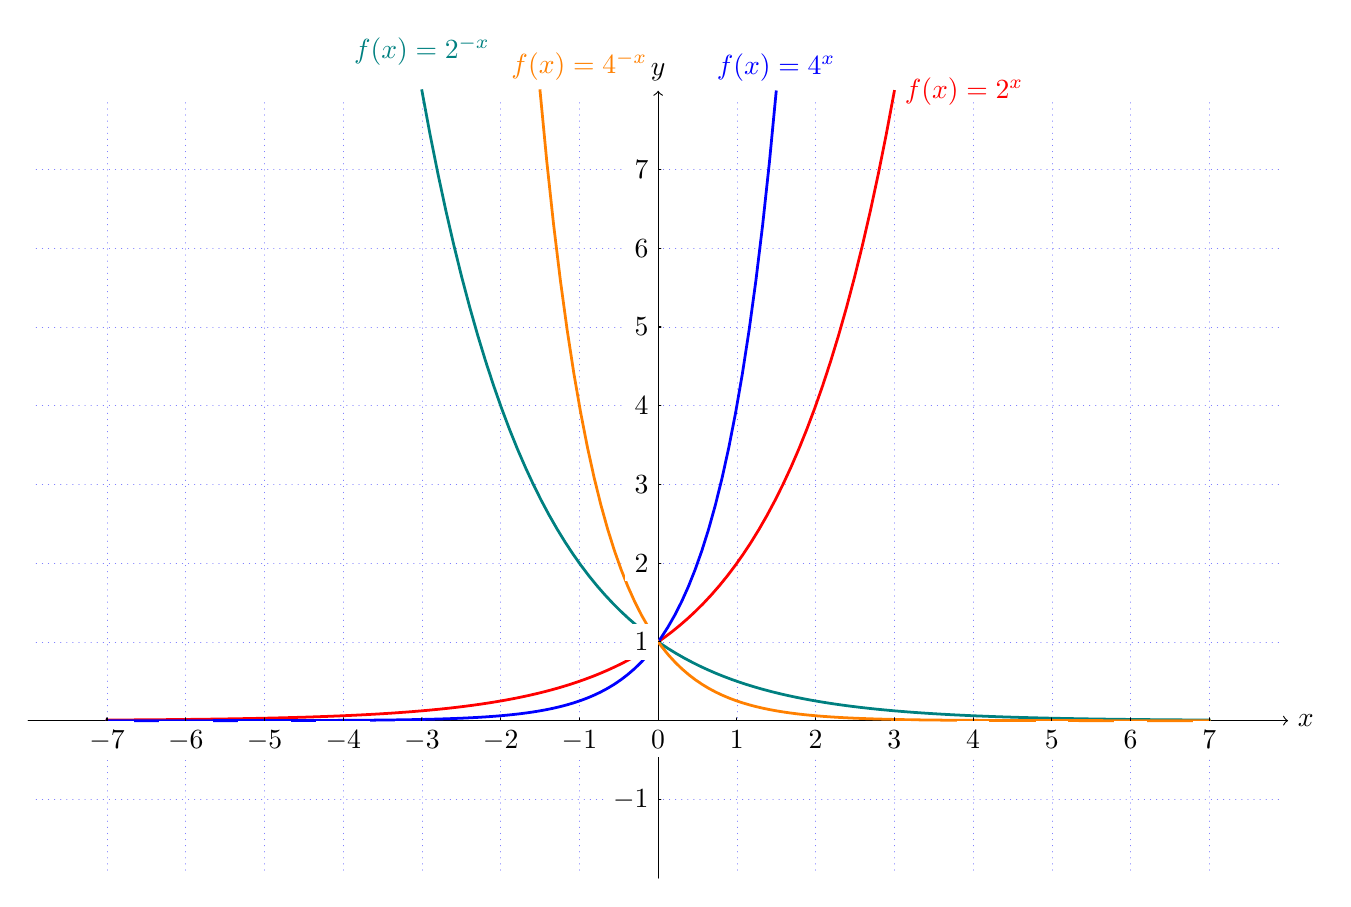
\begin{tikzpicture}[scale=1,cap=round]

% Styles
\tikzstyle{axes}=[]
\tikzstyle help lines=[color=blue!50,very thin,dotted]

% grid
\draw[style=help lines,step=1cm] (-7.9,-1.9) grid (7.9,7.9);

\draw[->] (-8,0) -- (8,0) node[right] {$x$};
\draw[->] (0,-2) -- (0,8) node[above] {$y$};

%\draw[fill,cyan](1,1)circle [radius=0.025];
%FUNCTIEVOORSCHRIFTEN


\draw[red,cap=rect,line width=1, opacity=1, domain=-7:3,samples=100] plot (\x, {
	pow(2,\x)	% <- plaats het functievoorschrift hier	
}) node[opacity=1,above,right]{$f(x)=2^x$};
%-------------------------------------------




\draw[blue,cap=rect,line width=1, opacity=1, domain=-7:1.5,samples=100] plot (\x, {
	pow(4,\x)	% <- plaats het functievoorschrift hier	
}) node[opacity=1,above]{$f(x)=4^x$};
%-------------------------------------------


\draw[teal,cap=rect,line width=1, opacity=1, domain=-3:7,samples=100] plot (\x, {
	pow(2,-\x)	% <- plaats het functievoorschrift hier	
}) node[opacity=1,,pos=0,xshift=-3cm,yshift=+8.5cm]{$f(x)=2^{-x}$};
%-------------------------------------------




\draw[orange,cap=rect,line width=1, opacity=1, domain=-1.5:7,samples=100] plot (\x, {
	pow(4,-\x)	% <- plaats het functievoorschrift hier	
}) node[opacity=1,above,pos=0,xshift=-1cm,yshift=+8cm]{$f(x)=4^{-x}$};
%-------------------------------------------


%legende



%getallen op de x-as en lijntjes   
\foreach \x/\xtext in {-7,-6,-5,-4,-3,-2,-1,0,1,2,3,4,5,6,7}
	\draw[xshift=\x cm] (0pt,1pt) -- (0pt,0pt) node[below,fill=white]
	{$\xtext$};,3
	
%getallen op de y-as en lijntjes  
%BEGIN LUS
\foreach \y/\ytext in {-1,1,2,3,4,5,6,7}
	\draw[yshift=\y cm] (1pt,0pt) -- (0pt,0pt) node[left,fill=white]
	{$\ytext$}; %EINDE LUS



\end{tikzpicture}
\end{center}

	
\end{figure}

%\gewonefiguur{width=7cm}{2_elem_rekenvaardigheden_B/inputs/exp}

Nulpunten
\begin{itemize}
	\item Er zijn geen nulpunten. De exponenti\"ele functie heeft geen snijpunten
	met de $x$-as. De $x$-as is de horizontale asymptoot.
	\item Het punt $(0,1)$ is het enige snijpunt met de $y$-as.
\end{itemize}

Tekenverloop

\begin{itemize}
	\item Alle functiewaarden $f(x)$ zijn strikt positief, de grafiek ligt
	overal boven de $x$-as.
\end{itemize}

\begin{voorbeeld}
$y=2^{x}$

Grafische voorstelling (stap1):
het grondtal is 2, en $2>0$,
dus krijgen we een stijgende functie. Het punt $(1,a)$ is hier dus
$(1,2)$ en behoort tot de functie ${\displaystyle y=2^{x}}$.


Nulpunten (stap2):
er zijn geen nulpunten. De $x$-as
wordt nooit gesneden. De $x$-as is de horizontale asymptoot. De $y$-as
wordt gesneden in het punt $(0,1)$.


Tekenverloop (stap3) %

\begin{tabel}{}
\begin{tabular}{c|c}
	$x$ & $\longrightarrow\mathbb{R}$\\
	\hline 
	\multirow{1}{*}{$2^{x}$} & + \\
\end{tabular}

\end{tabel}

Grafiek (stap4) 
%TODO figuur vervangen
\begin{figure}[H]
	\input{2_elem_rekenvaardigheden_B/Fig_module_2_1_10_exponentiele_functie_2}	
\end{figure}

\end{voorbeeld}

